\lyxframe{Label Propagation Algorithm for Graph Connected Component Algorithm}

\only<1>{
\centering
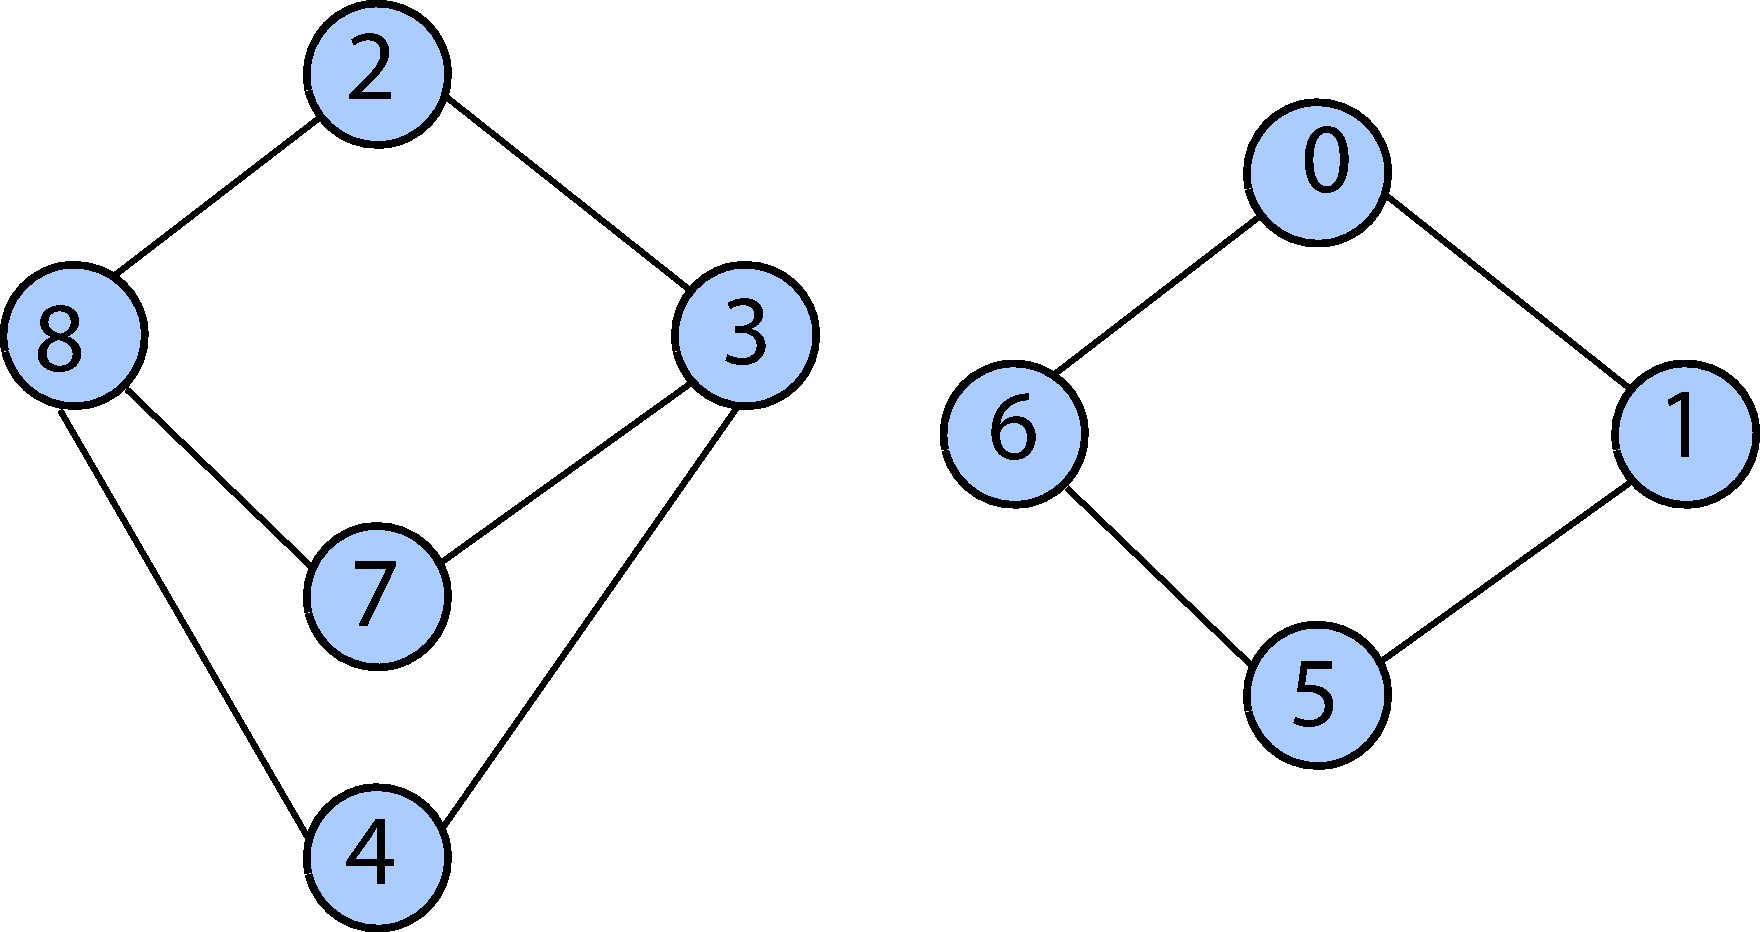
\includegraphics[height=0.4\textheight]{images/base}
}
\only<2>{
\centering
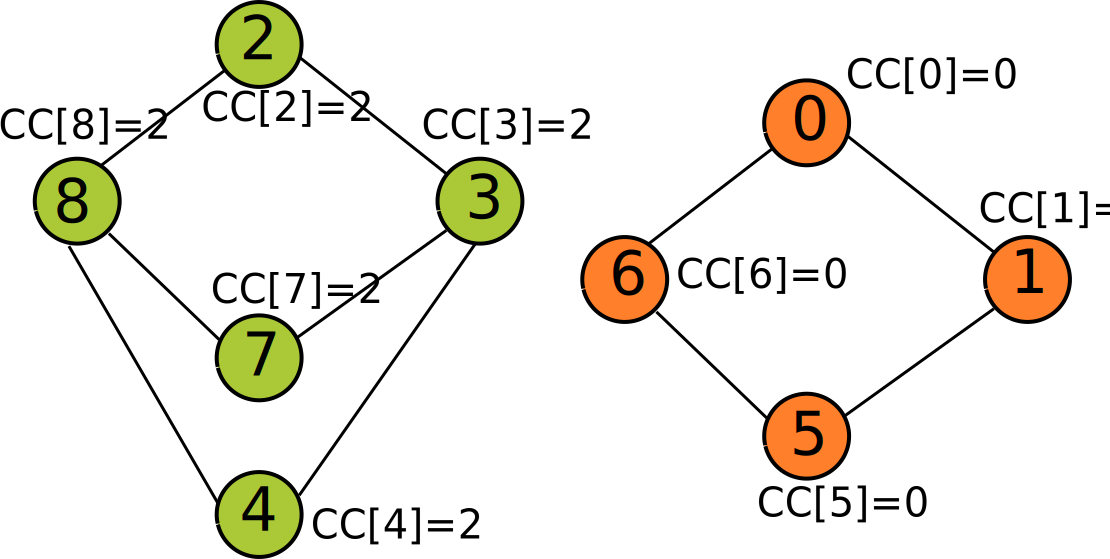
\includegraphics[height=0.4\textheight]{images/lp/lp-4}
}

\begin{block}{Graph Connected-component Problem}
We seek to find number of connected-components in the graph and which connected component 
each vertex belongs to.
\begin{itemize}
\item Used for community detection, centrality analytics and streaming graph analytics. 
\item Label propagation is highly suited for parallel computing. 
\end{itemize}
\end{block}
\lyxframeend{}
%%%%%%%%%%%%%%%%%%%%%%%%%%%%%%%%%%%%%%%%%%%%%%%%%%%%%%%%%
\lyxframe{Label Propagation Algorithm}

\only<1>{
\centering
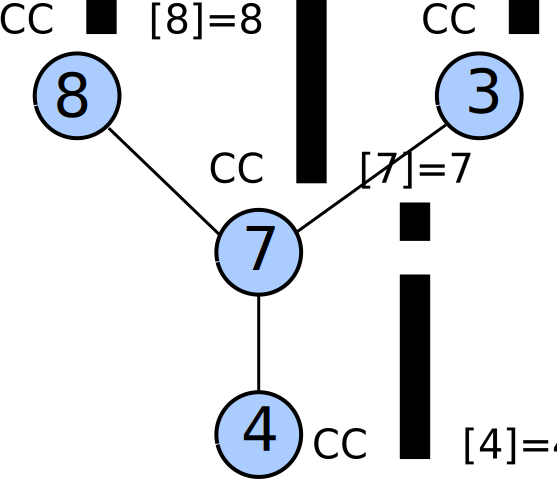
\includegraphics[height=0.4\textheight]{images/lp-initialize}

}
\only<2>{
\centering
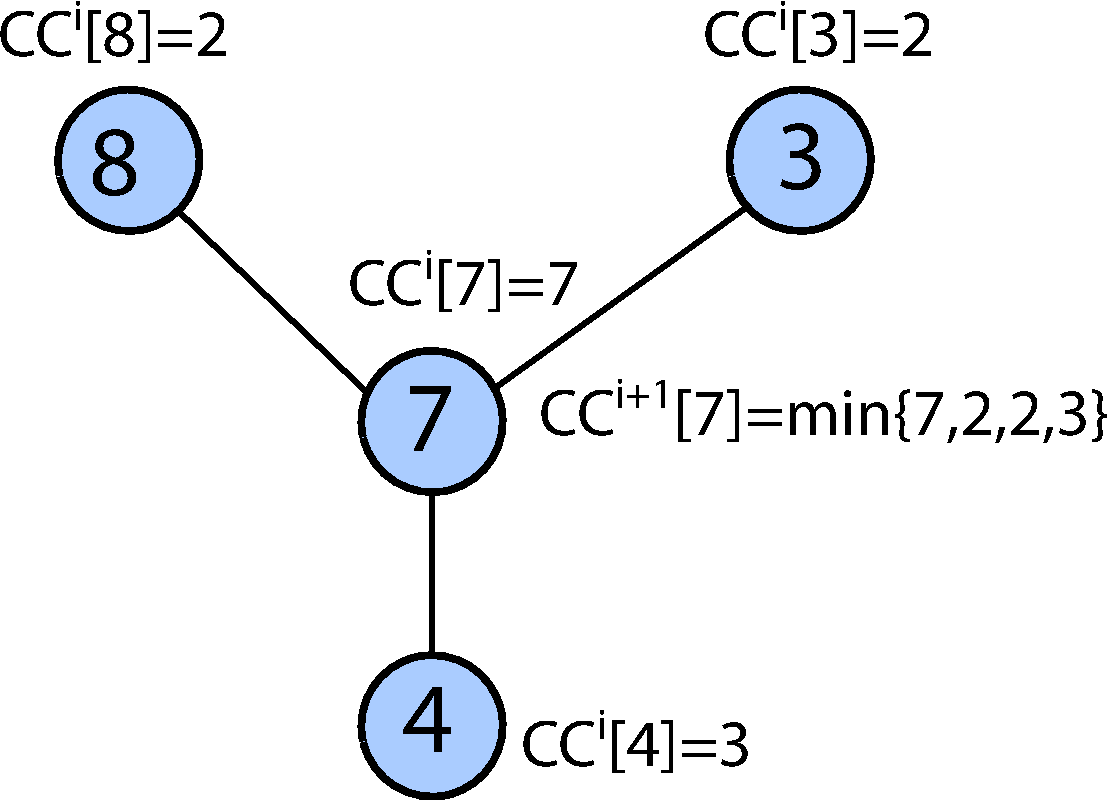
\includegraphics[height=0.4\textheight]{images/lp-update}

}


\begin{itemize}
\item Propagates the minimum label in the connected component.
\item We maintain a \emph{label} array $CC$ for each vertex.
\item $CC$ is initialized to vertex id for each vertex.
\item In each iteration, each vertex calculates minimum label among all near-neighbours $\mathcal{N}(v)=v\cup adj(v)$
\[ CC^{i}[v] = \min_{u \in \mathcal{N}(v)} CC^{i-1}[u]. \]
\item Iteration terminates when no change occur in an iteration.

\end{itemize}
\lyxframeend{}

%%%%%%%%%%%%%%%%%%%%%%%%%%%%%%%%%%%%%%%%%%%%%%%%%%%%%%%%%
\lyxframe{Label Propagation Algorithm- Example}

\only<1>{
\centering
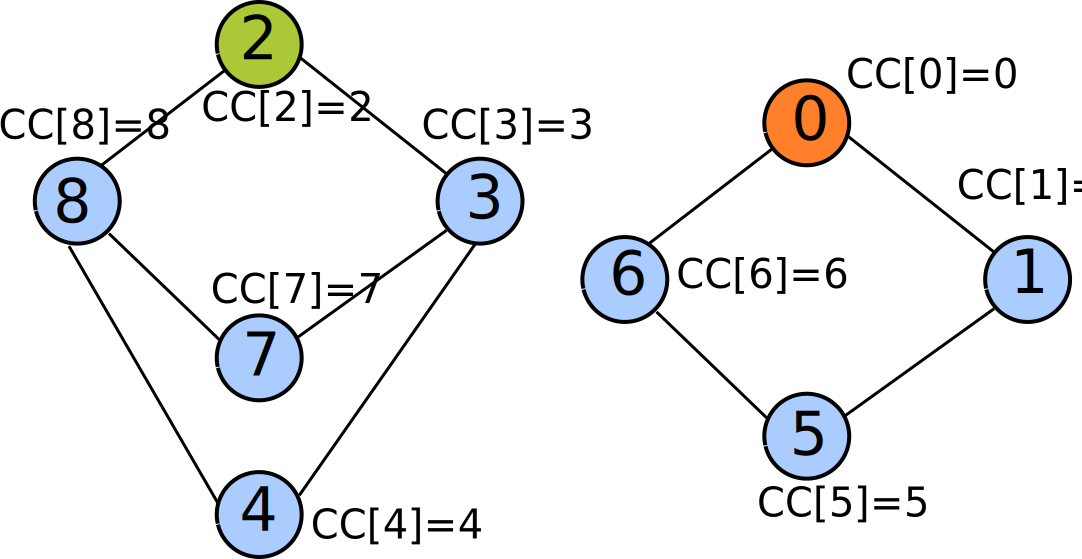
\includegraphics[height=0.4\textheight]{images/lp/lp-1}

}
\only<2>{
\centering
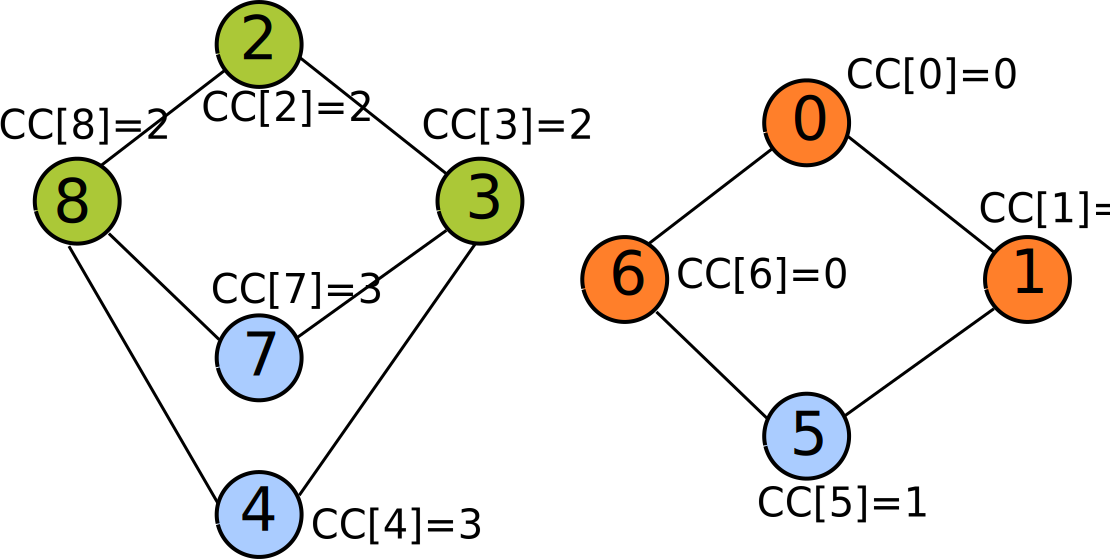
\includegraphics[height=0.4\textheight]{images/lp/lp-2}

}
\only<3>{
\centering
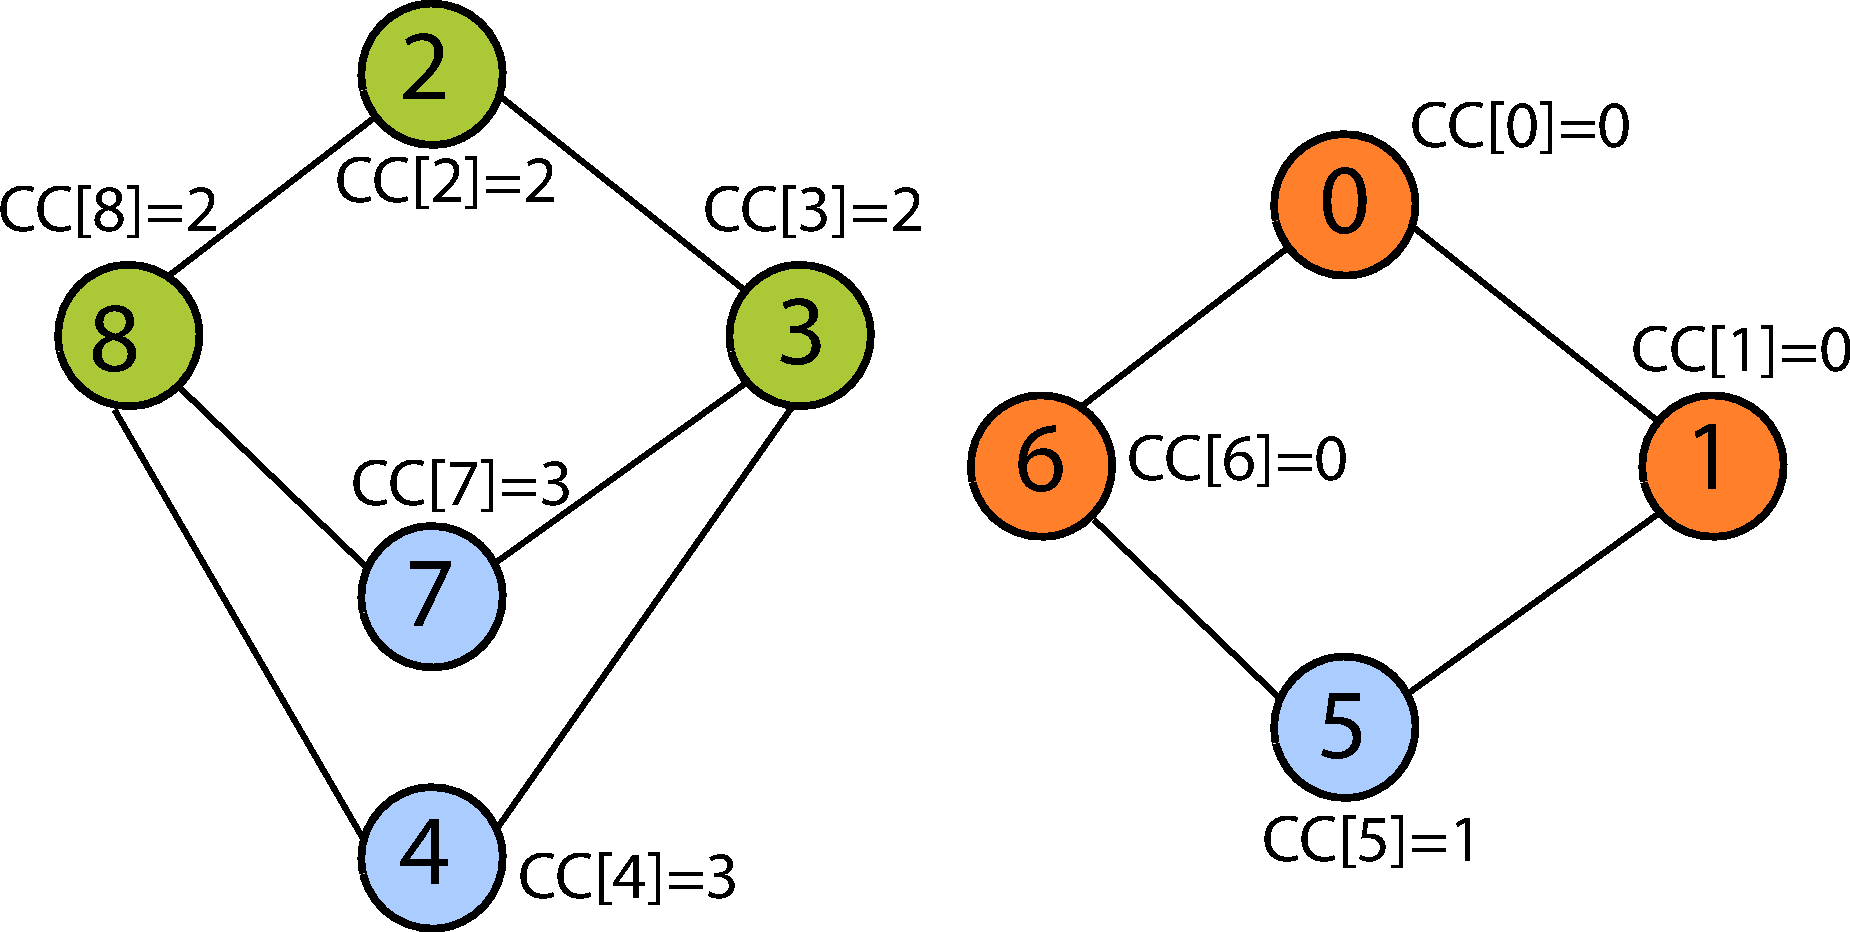
\includegraphics[height=0.4\textheight]{images/lp/lp-3}

}
\only<4>{
\centering
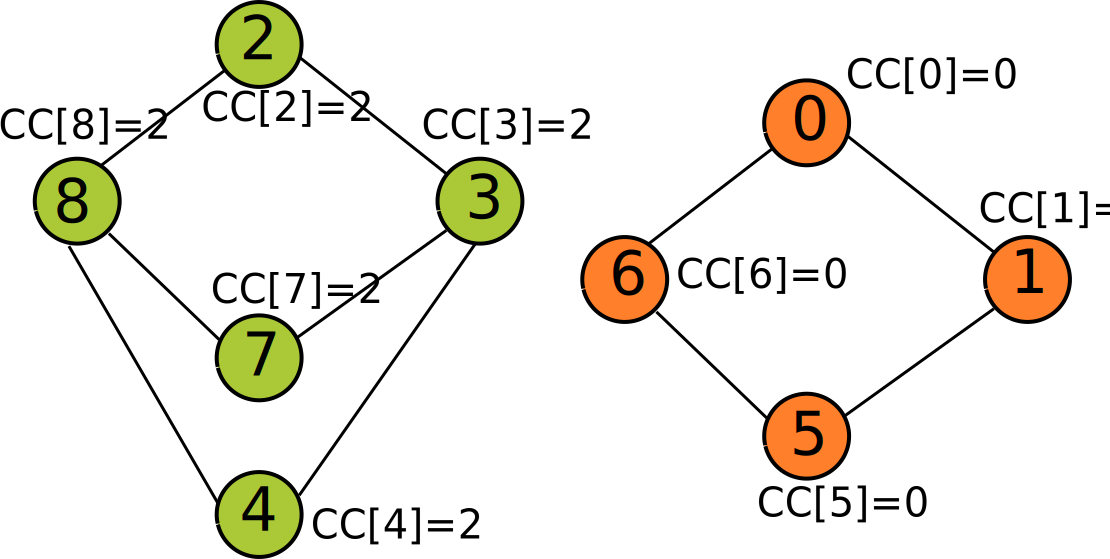
\includegraphics[height=0.4\textheight]{images/lp/lp-4}

}

\begin{itemize}
\item Minimum label in the connected component (shown in {\color{green} green} and {\color{orange} orange} ) propagates to all the vertex in the connected components. 
\end{itemize}
\lyxframeend{}

%%%%%%%%%%%%%%%%%%%%%%%%%%%%%%%%%%%%%%%%%%%%%%%%%%%%%%%%%
\lyxframe{State of Label Propagation Algorithm}
\begin{columns}
% change following images
\begin{column}{0.5\textwidth}  %%<--- here
    \only<1>{
\centering
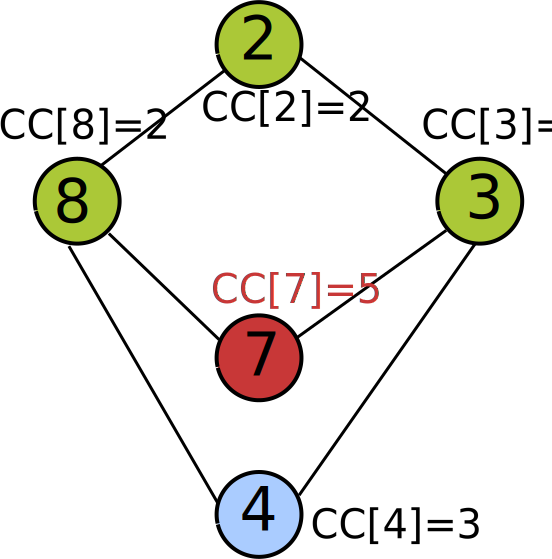
\includegraphics[height=0.5\textheight]{images/fault-corrected/fault-corrected-1}

}

\end{column}

\begin{column}{0.5\textwidth}
   \begin{itemize}
   \item<1-> $CC$ vector defines the state of the LP algorithm.
   
   \end{itemize}
\end{column}

\end{columns}


\lyxframeend{}

%%%%%%%%%%%%%%%%%%%%%%%%%%%%%%%%%%%%%%%%%%%%%%%%%%%%%%%%%
\lyxframe{Single Fault In Label Propagation Algorithm- Fault Correction}
\begin{columns}
\begin{column}{0.5\textwidth}

\only<1>{
\centering
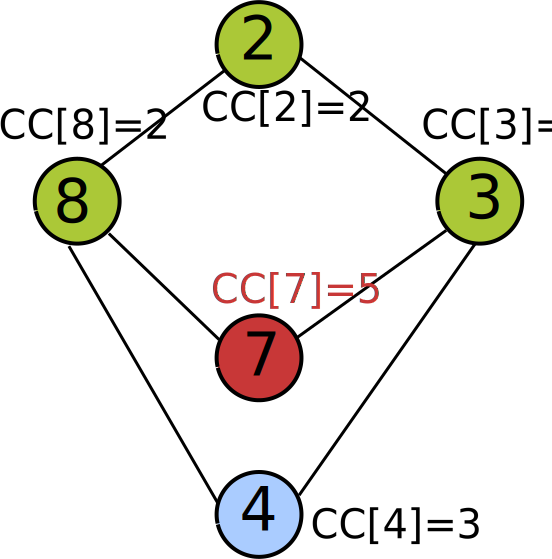
\includegraphics[height=0.5\textheight]{images/fault-corrected/fault-corrected-1}

}
\only<2>{
\centering
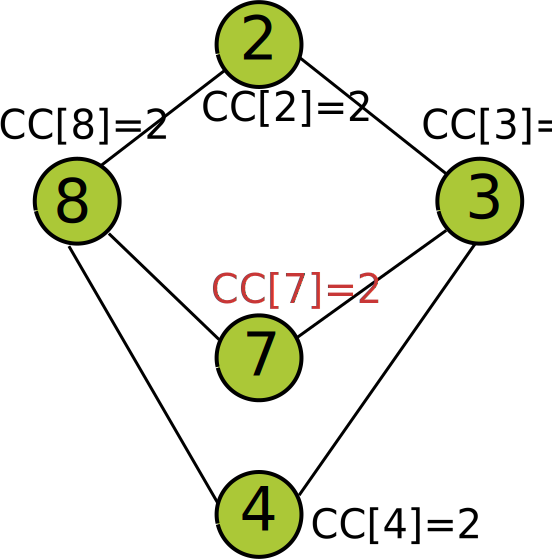
\includegraphics[height=0.5\textheight]{images/fault-corrected/fault-corrected-2}

}
\end{column}
%%%%%%%%%%%% == column == %%%%%%%%%%%%
\begin{column}{0.5\textwidth}
\begin{itemize}
   \item $CC$ value can be corrupted due to hardware faults.
   \item Depending on error caused by the fault, some error can be corrected by the algorithm.
   \item Example: corrupted $CC[v]$ value is arbitrarily high.
   \item Such faults do not cause the algorithm to transition to an invalid state, but they can still cause delay in convergence. 
   \end{itemize}
\end{column}

\end{columns}
\lyxframeend{}

%%%%%%%%%%%%%%%%%%%%%%%%%%%%%%%%%%%%%%%%%%%%%%%%%%%%%%%%%

\lyxframe{Single Fault In Label Propagation Algorithm- Fault Propagation}
\begin{columns}
%%%%%%%%%%%% == column == %%%%%%%%%%%%
\begin{column}{0.5\textwidth}
\only<1>{
\centering
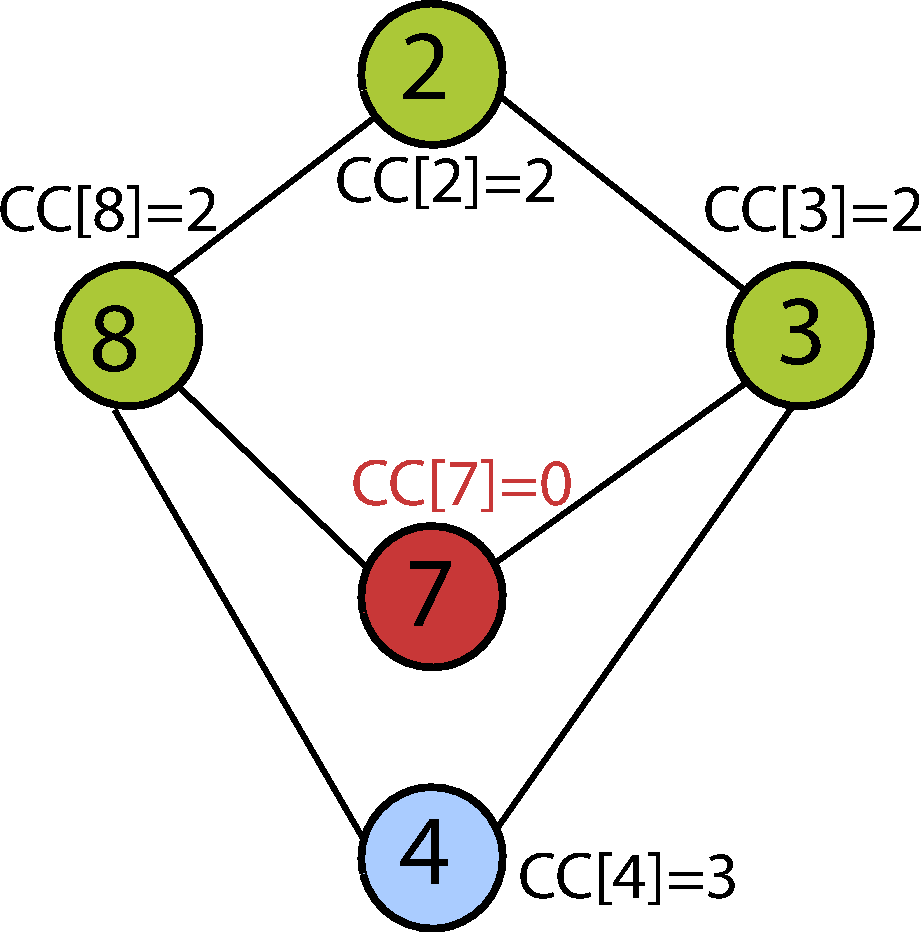
\includegraphics[height=0.5\textheight]{images/fault-propagated/fault-propagated-1}

}
\only<2>{
\centering
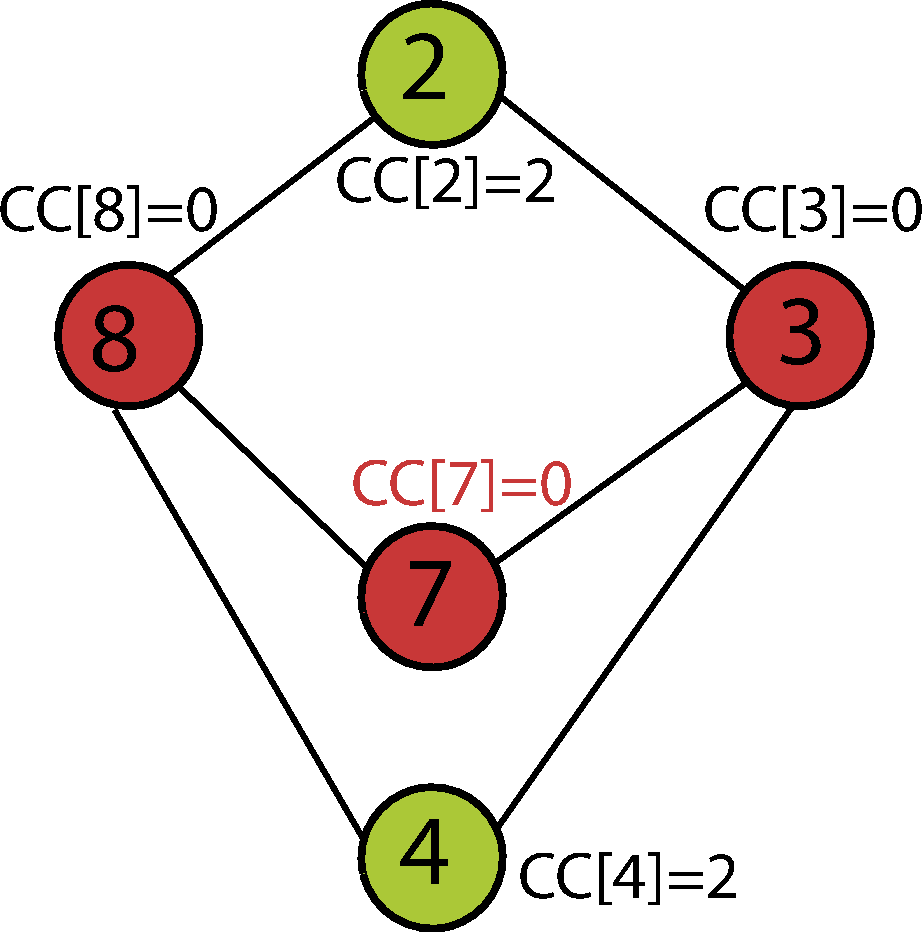
\includegraphics[height=0.5\textheight]{images/fault-propagated/fault-propagated-2}

}
\only<3>{
\centering
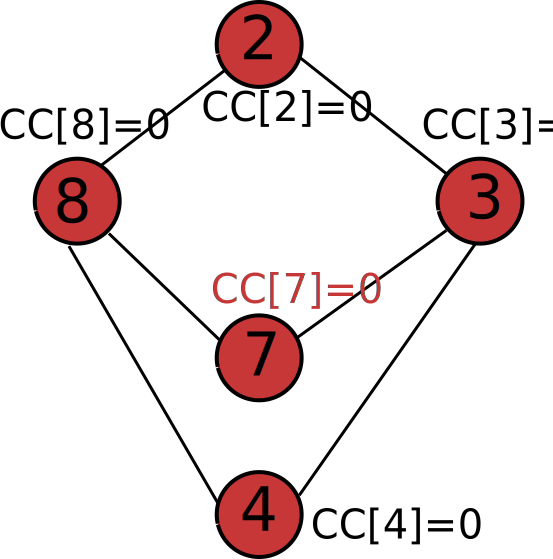
\includegraphics[height=0.5\textheight]{images/fault-propagated/fault-propagated-3}

}
\end{column}
%%%%%%%%%%%% == column == %%%%%%%%%%%%
\begin{column}{0.5\textwidth}
\begin{itemize}
	\item If the fault causes a corruption such $CC[v]$ is changed to a values lower than the $CC^{\infty}[v]$, the error will propagate to all the other vertex in the connected component. 
	\item Such faults do not cause the algorithm to transition to an invalid state.
	\item \color{red} It is not computationally easy to determine whether a given snapshot of $CC$ is a valid state. 
\end{itemize}
\end{column}

\end{columns}
\lyxframeend{}

%%%%%%%%%%%%%%%%%%%%%%%%%%%%%%%%%%%%%%%%%%%%%%%%%%%%%%%%%
\lyxframe{Valid States}
\begin{block}{Classification of different corruption}
Consider following three cases:
\begin{enumerate}
	\item<1-> $CC[v]>v$: Easy to detect and automatically corrected in most cases.  
	\item<2-> $CC^{\infty}[v] \leq CC[v] \leq v$: ??
	\item<3-> {\color{red} $CC[v] < CC^{\infty}[v]$: Will definitely cause algorithm to fail. }
\end{enumerate}
\end{block}


\onslide<4->\begin{theorem}

A connected component array $CC$ is a valid state---i.e.,
a fault-free execution of algorithm  starting from $CC$ will converge to the correct solution---if, for all vertices $v$, 
\[ CC^{\infty}[v] \leq CC[v] \leq v.
\]

\end{theorem} 
% \pause

\onslide<5->
\centering 
\color{red} The only problem is, $CC^{\infty}[v]$---being the solution, is not known. 

\lyxframeend{}
%%%%%%%%%%%%%%%%%%%%%%%%%%%%%%%%%%%%%%%%%%%%%%%%%%%%%%%%%

\lyxframe{Self-correcting Label Propagation Algorithm- 1 }
We apply principle of self-correction to resolve the apparent difficulty in verifying state validity.
\begin{itemize}
\item<2-> We assume the previous state $CC^{i-1}$ is a valid one.
\item<3-> Checking 
\[ CC^{i}[v] = \min_{u \in \mathcal{N}(v)} CC^{i-1}[u], \]
 where  $\mathcal{N}(v) \equiv v \cup adj(v)$ is the immediate \emph{neighborhood} of $v$, {\color{red} will require re-computing entire iteration.}
\item<4-> We show that $CC^{i}[v]$ is still a valid value even if we can relax the minimization criterion to
\[
CC^{i}[v] \in \{ CC^{i-1}[u] \, | \, u \in \mathcal{N}(v) \}, %CC^{i-1}[v]_{adj} \},
\] 

\end{itemize}

\lyxframeend{}

%%%%%%%%%%%%%%%%%%%%%%%%%%%%%%%%%%%%%%%%%%%%%%%%%%%%%%%%%
\lyxframe{Self-correcting Label Propagation Algorithm- 2}
\begin{theorem}
Given a valid state for the previous iteration, $CC^{i-1}$, the current connected component array $CC^{i}$ is a valid state if for all vertices $v$, $CC^{i}$ satisfies these conditions:
\begin{enumerate}
\item $CC^{i}[v] \leq v$; and
\item there exists a vertex $u$ such that $CC^{i}[v]=CC^{i-1}[u]$ and $u \in \mathcal{N}(v)$. %$u \in 
\end{enumerate}
\end{theorem}

\pause
\begin{block}{ Cost of Direct Verification}
\begin{itemize}
\item Verifying $CC^{i}[v] \leq v$ requires $\bigO{V}$ operation.
\item Verifying second condition requires traversing adjacency list for each vertex $v$, that will require
$\bigO{V+E}$ operations, \color{red} as costly as an LP iteration.
\end{itemize}

\end{block}


\lyxframeend{}

%%%%%%%%%%%%%%%%%%%%%%%%%%%%%%%%%%%%%%%%%%%%%%%%%%%%%%%%%
\lyxframe{Validity Checking: Auxiliary Data Structure- 1}
\begin{columns}
%% resize the above figure
\begin{column}{0.5\textwidth}
\only<1>{
\centering
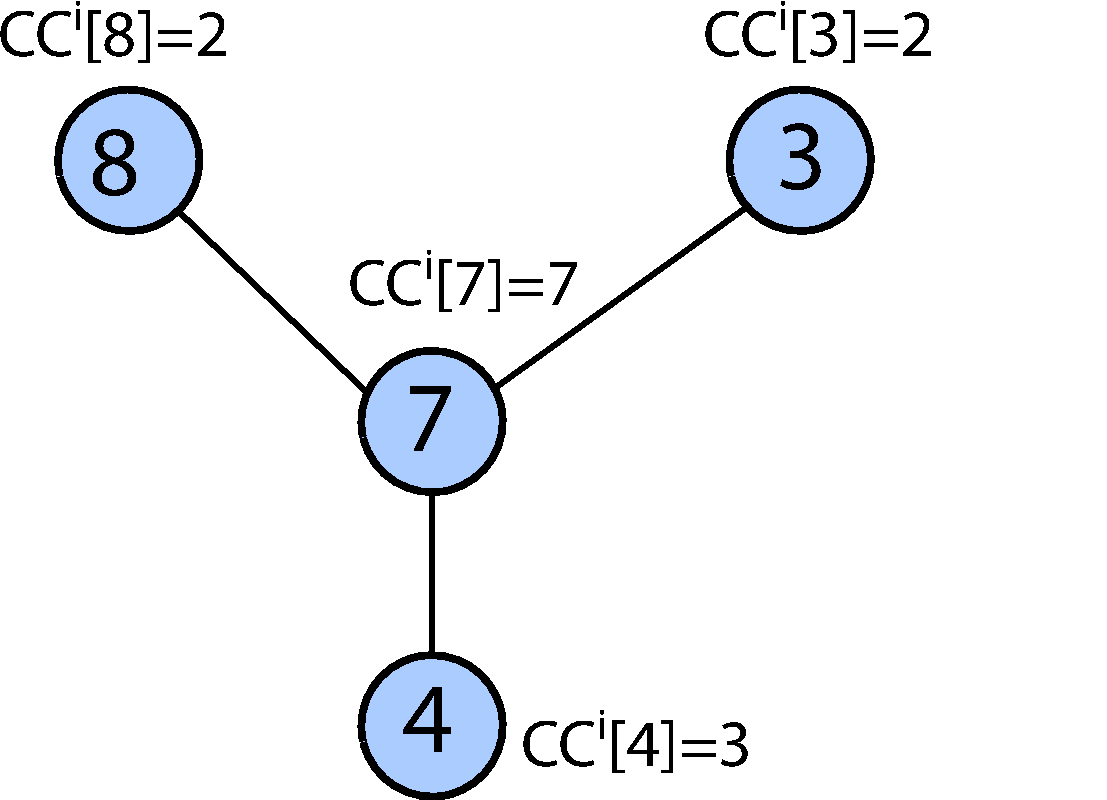
\includegraphics[height=0.5\textheight]{images/parent/parent-1}

}
\only<2->{
\centering
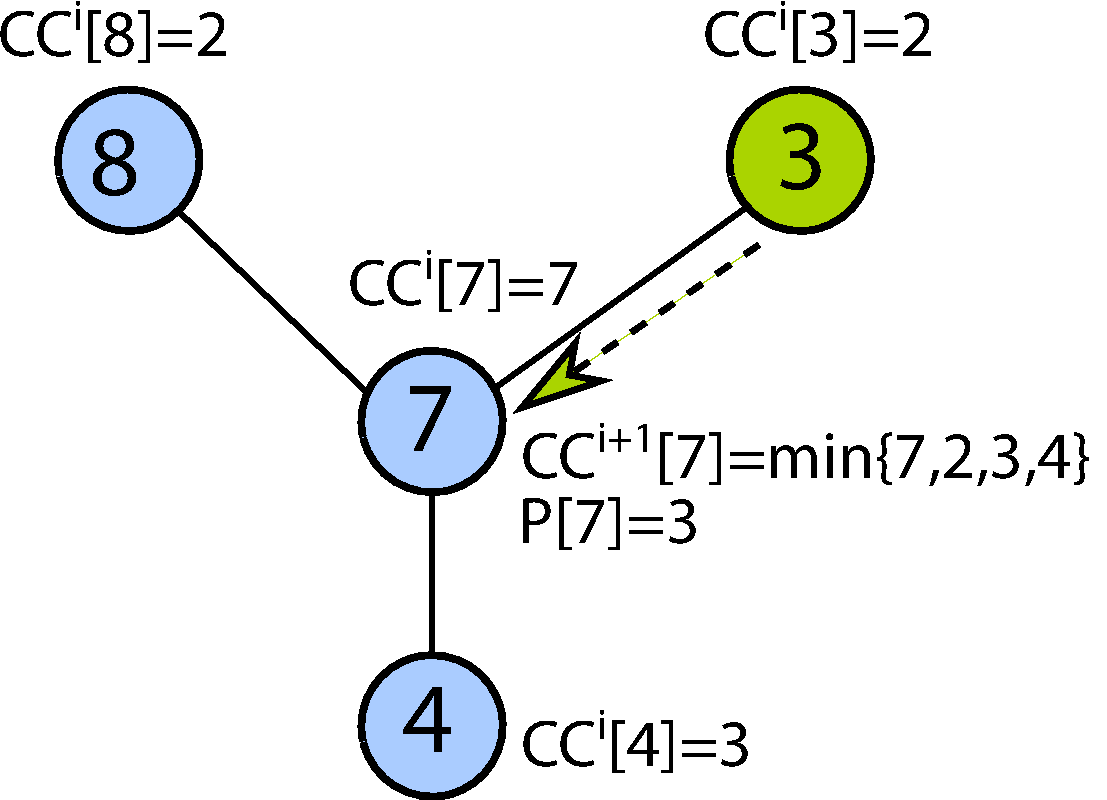
\includegraphics[height=0.5\textheight]{images/parent/parent-2}

}
\end{column}

\begin{column}{0.5\textwidth}
\begin{exampleblock}{Parent Array}
\begin{itemize}
\item Parent array $P$: We may store store information of the vertex $u$ that caused the last change in $CC[v]$.
\item If $u= P[v]$ then $CC^{i}[v] = CC^{i-1}[P[v]]$, can be verified in $\bigO{V}$ operations for all vertex.
\item Storing $P$ requires an memory of $\bigO{V}$.
 \end{itemize}
\end{exampleblock}

\onslide<3->
\begin{alertblock}{Corruption of $P$}

\begin{itemize}
\item $P$ also can be corrupt.
\item $P$ is valid if $P[v] \in \mathcal{N}(v)$ for all vertex $v$.
\item \color{red} Checking $P$ is valid requires again $\bigO{V+E}$ operations.
\end{itemize}
\end{alertblock}
\end{column}
\end{columns}
\lyxframeend{}

%%%%%%%%%%%%%%%%%%%%%%%%%%%%%%%%%%%%%%%%%%%%%%%%%%%%%%%%%
\lyxframe{Validity Checking: Auxiliary Data Structure- 2}
\begin{columns}
\begin{column}{0.5\textwidth}
\centering
\only<1>{
\centering
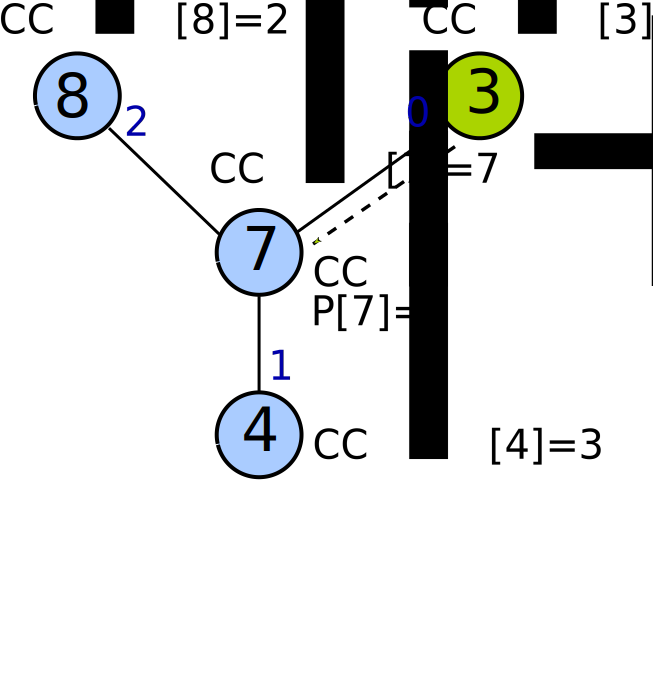
\includegraphics[height=0.5\textheight]{images/parent/new-parent-1}

}
\only<2>{
\centering
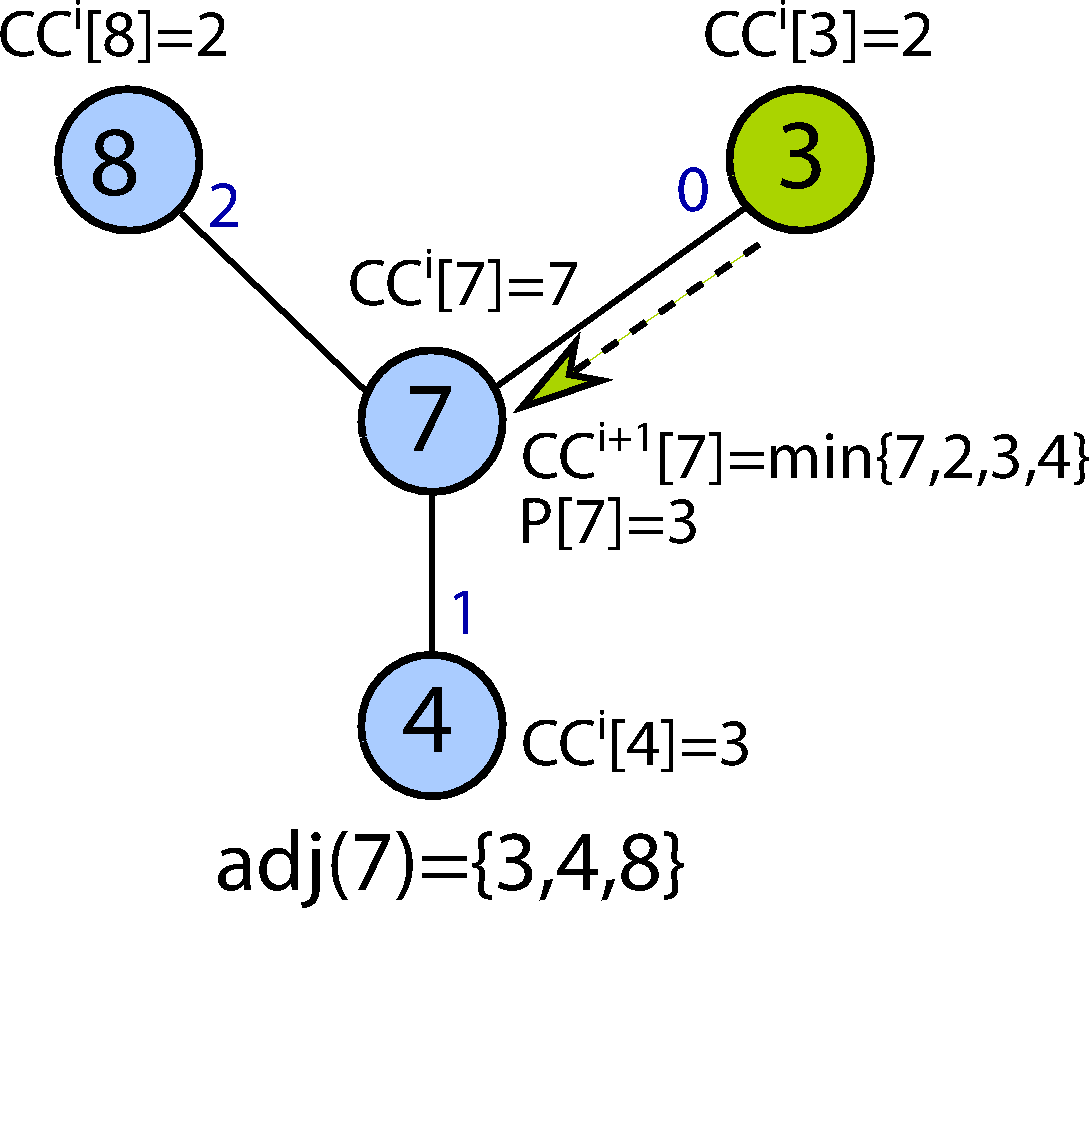
\includegraphics[height=0.5\textheight]{images/parent/new-parent-2}

}
\only<3>{
\centering
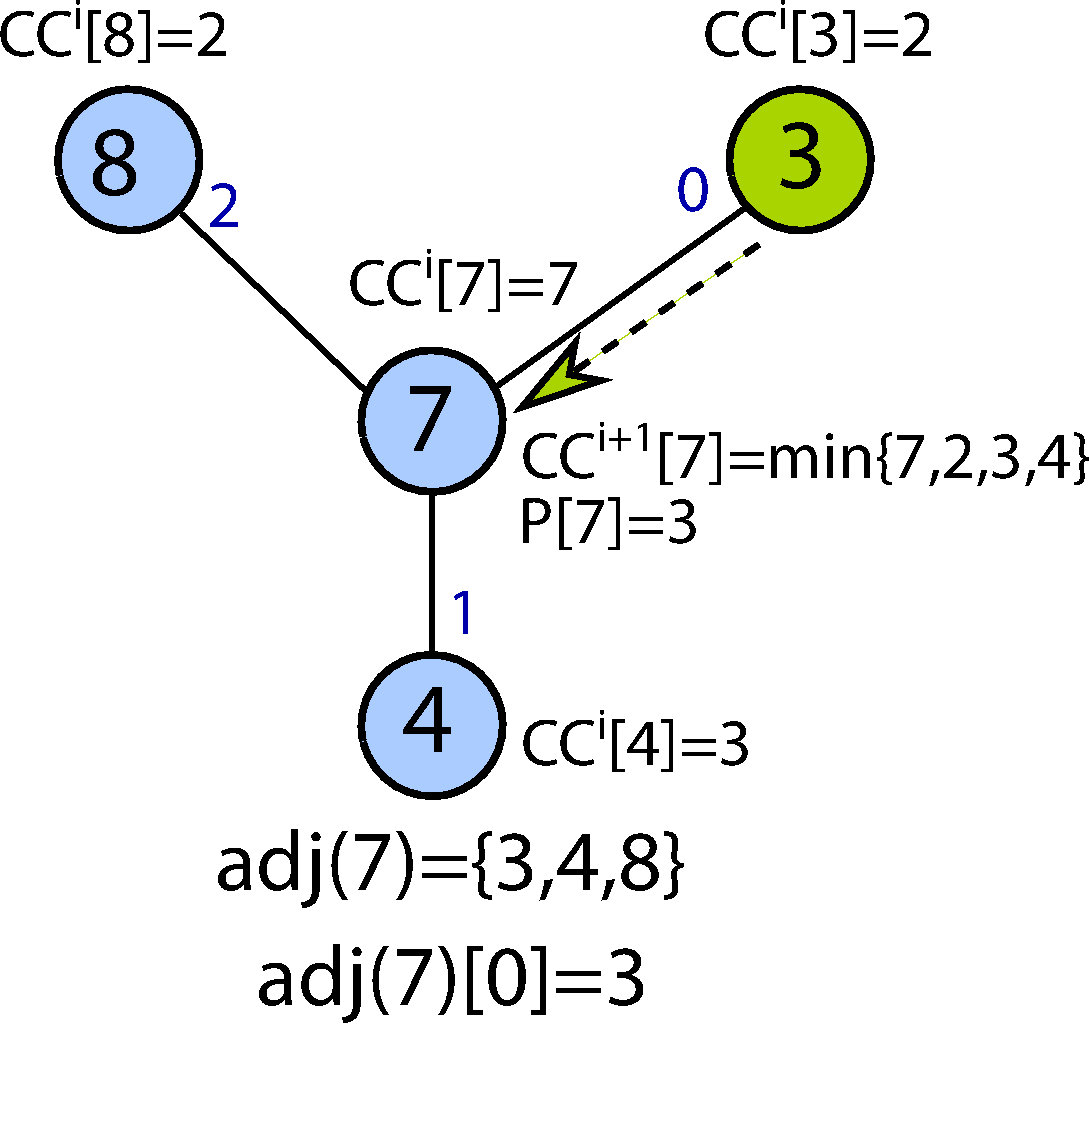
\includegraphics[height=0.5\textheight]{images/parent/new-parent-3}

}
\only<4->{
\centering
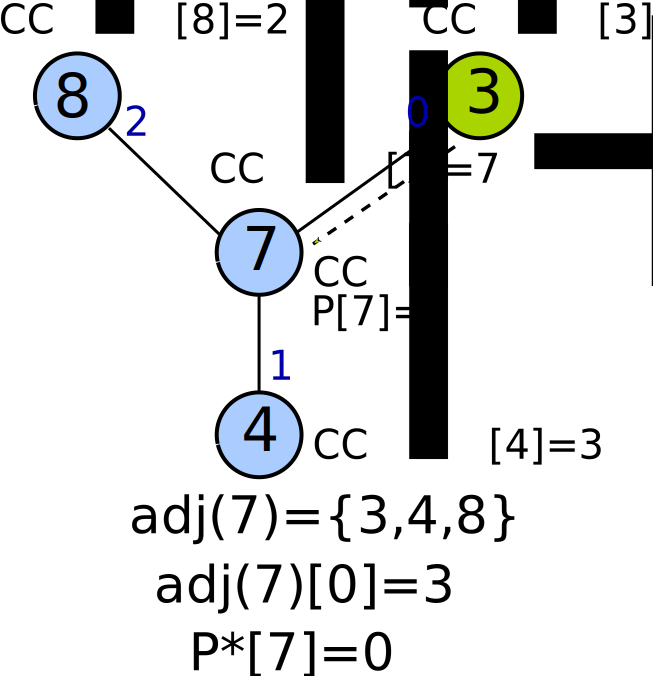
\includegraphics[height=0.5\textheight]{images/parent/new-parent-4}

}
\end{column}
\begin{column}{0.5\textwidth}
\begin{block}{Index Based Parent Array}
\begin{itemize}
\item<1-> Instead of storing $u$, we store index of $u$ in $adj(v)$.
\begin{align*}
       &E & \leftarrow & adj(v) \\
		&u   & \leftarrow & E[k]\\
	&P^{*}[v]   & \leftarrow & k  
\end{align*}
\item<5-> When $P[v]=v$, then  $P^{*}[v]=-1$
\item<6-> $CC^{i}[v] = CC^{i-1}[P[v]]$ reduces to 
\[
	CC^{i}[v] = CC^{i-1}[ adj(v)[P^{*}[v]]];
\]
{\color{dpg} $\bigO{V}$ operations. }% \end{itemize}
% \end{block}

% \begin{block}{}
% \begin{itemize}
% \item $P^{*}$ also requires $\bigO{V}$ memory.
\item<7-> Validity of $P^{*}$:  $-1 \leq P^{*}[v] < |adj(v)| $; 
{\color{dpg}  $\bigO{V}$ operations.}
\end{itemize}
\end{block}
\end{column}
\end{columns}
\lyxframeend{}
%%%%%%%%%%%%%%%%%%%%%%%%%%%%%%%%%%%%%%%%%%%%%%%%%%%%%%%%%

\lyxframe{Fault Detection and Correction}
\begin{exampleblock}{Invalid State Detection}
In summary, the set of conditions to check for each vertex are:
\begin{align*}
\begin{split}
CC^{i}[v] 		&\leq v;  \\
 -1 			&\leq P^{*}[v] < |adj(v)|; \text{and} \\
CC^{i}[v]		&= \begin{cases}
v & \text{ if } P^{*}[v] = -1  \\
CC^{i-1}[ adj(v)[P^{*}[v]]] & \text{ if } P^{*}[v]\ne -1
\end{cases}.
\end{split} 
\end{align*}
\end{exampleblock}

\pause 

\begin{alertblock}{State Correction}
For any vertex $v$, if state validity check fails then, we recompute  $CC^{i}[v]$.
\end{alertblock}
\lyxframeend{}

%%%%%%%%%%%%%%%%%%%%%%%%%%%%%%%%%%%%%%%%%%%%%%%%%%%%%%%%%
\lyxframe{Overhead of Self-correcting Label-propagation Algorithm}
\begin{center}
\begin{tabular}{l|c}
\toprule 
      Overhead           & Asymptotic Complexity     \\
\midrule                  
Fault detection        & $\mathcal{O}(|V|)$      \\
Fault correction       & $\mathcal{O}(f|E|/|V|)$ \\
Auxiliary data structure     & $\mathcal{O}(|V|)$      \\
\bottomrule 
\end{tabular}
\end{center}
\begin{itemize}
\item Number of state corrections $f$, can be significantly less than faults occurred.
\item Fault detection and correction needs to be done in a guaranteed reliable mode.
\end{itemize}

\lyxframeend{}